\documentclass{standalone}

\usepackage{amssymb}
\usepackage{amsthm}
\usepackage{amsmath}


\usepackage{tikz}
\usetikzlibrary{shapes,backgrounds,calc,patterns}
\usepackage{venndiagram}


\begin{document}
    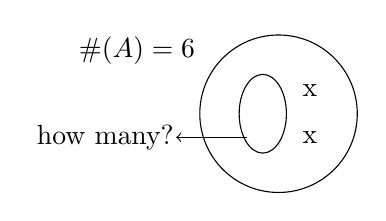
\begin{tikzpicture}
\draw (-1,0) circle (1);

\node at (-.6,.3) {x};
\node at (-.6,-.3) {x};
\draw (-1.2,0) ellipse (.3 and .5);
\draw[->] (-1.4,-.3) -- (-2.3,-.3);
\node at (-3.2,-.3) {how many?};
\node at (-2.8,.8) {\(\#(A)=6\)};
\end{tikzpicture}
\end{document}